\documentclass[11pt,a4paper]{ivoa}
\input tthdefs

\title{ProposalDM: A Datamodel for Observation Proposals}

% see ivoatexDoc for what group names to use here; use \ivoagroup[IG] for
% interest groups.
\ivoagroup{Data Models}

\author[????URL????]{Paul Harrison}

\editor{Paul Harrison}

% \previousversion[????URL????]{????Concise Document Label????}
\previousversion{This is the first public release}
       

\begin{document}
\begin{abstract}
This document and associated files define a data model in VO-DML that is intended to be suitable for exchanging
    information pertaining to making observation proposals. It is envisaged that the model will be useful in two scenarios.
\begin{itemize}
    \item transferring information between different Observatories' application processes.
    \item observatory scheduling systems being able to automatically extract source lists.
\end{itemize}
\end{abstract}


\section*{Acknowledgments}

Work on this standard is partially funded by the Opticon RadioNet Pilot project within the Horizon2020 programme, contract no. 101004719.

\section*{Conformance-related definitions}

The words ``MUST'', ``SHALL'', ``SHOULD'', ``MAY'', ``RECOMMENDED'', and
``OPTIONAL'' (in upper or lower case) used in this document are to be
interpreted as described in IETF standard RFC2119 \citep{std:RFC2119}.

The \emph{Virtual Observatory (VO)} is a
general term for a collection of federated resources that can be used
to conduct astronomical research, education, and outreach.
The \href{https://www.ivoa.net}{International
Virtual Observatory Alliance (IVOA)} is a global
collaboration of separately funded projects to develop standards and
infrastructure that enable VO applications.


\section{Introduction}


The concept of

https://www.eso.org/sci/meetings/2018/proposal-tools-workshop.html

Inspired by Alan Bridger and Bryan Butler "The ALMA/EVLA project data model: steps toward a common project
description for astronomy", Proc. SPIE 7019, Advanced Software and Control for Astronomy II, 70190P (14 July 2008);
https://doi.org/10.1117/12.789262

\subsection{Role within the VO Architecture}

\begin{figure}
\centering

% As of ivoatex 1.2, the architecture diagram is generated by ivoatex in
% SVG; copy ivoatex/archdiag-full.xml to role_diagram.xml and throw out
% all lines not relevant to your standard.
% Notes don't generally need this.  If you don't copy role_diagram.xml,
% you must remove role_diagram.pdf from SOURCES in the Makefile.

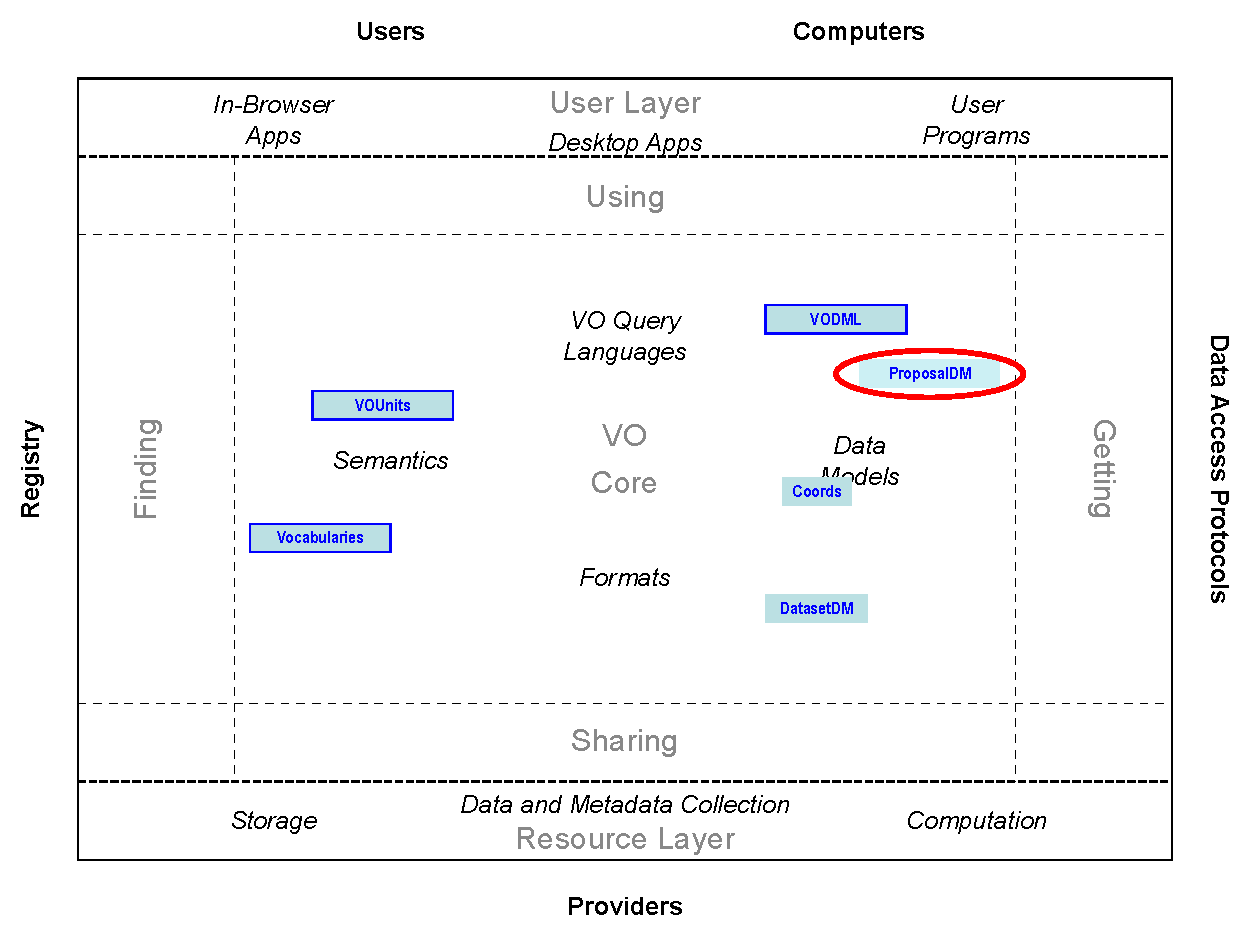
\includegraphics[width=0.9\textwidth]{role_diagram.pdf}
\caption{Architecture diagram for this document}
\label{fig:archdiag}
\end{figure}

Fig.~\ref{fig:archdiag} shows the role this document plays within the
IVOA architecture \citep{2010ivoa.rept.1123A}.

\section{The Model}

\appendix
\section{Changes from Previous Versions}

No previous versions yet.  
% these would be subsections "Changes from v. WD-..."
% Use itemize environments.


% NOTE: IVOA recommendations must be cited from docrepo rather than ivoabib
% (REC entries there are for legacy documents only)
\bibliography{ivoatex/ivoabib,ivoatex/docrepo}


\end{document}
